\subsection{Layer restoring performance--aware deduplication}
\label{sec:dedup-desgin}

We now describe \sysname's layer restoring performance--aware deduplication 
 (i.e., \sysname's~\dedupname) system design. 

\subsubsection{When to deduplicate layers?}

\begin{figure*}[t]
		\begin{minipage}{0.21\linewidth}
			\centering
			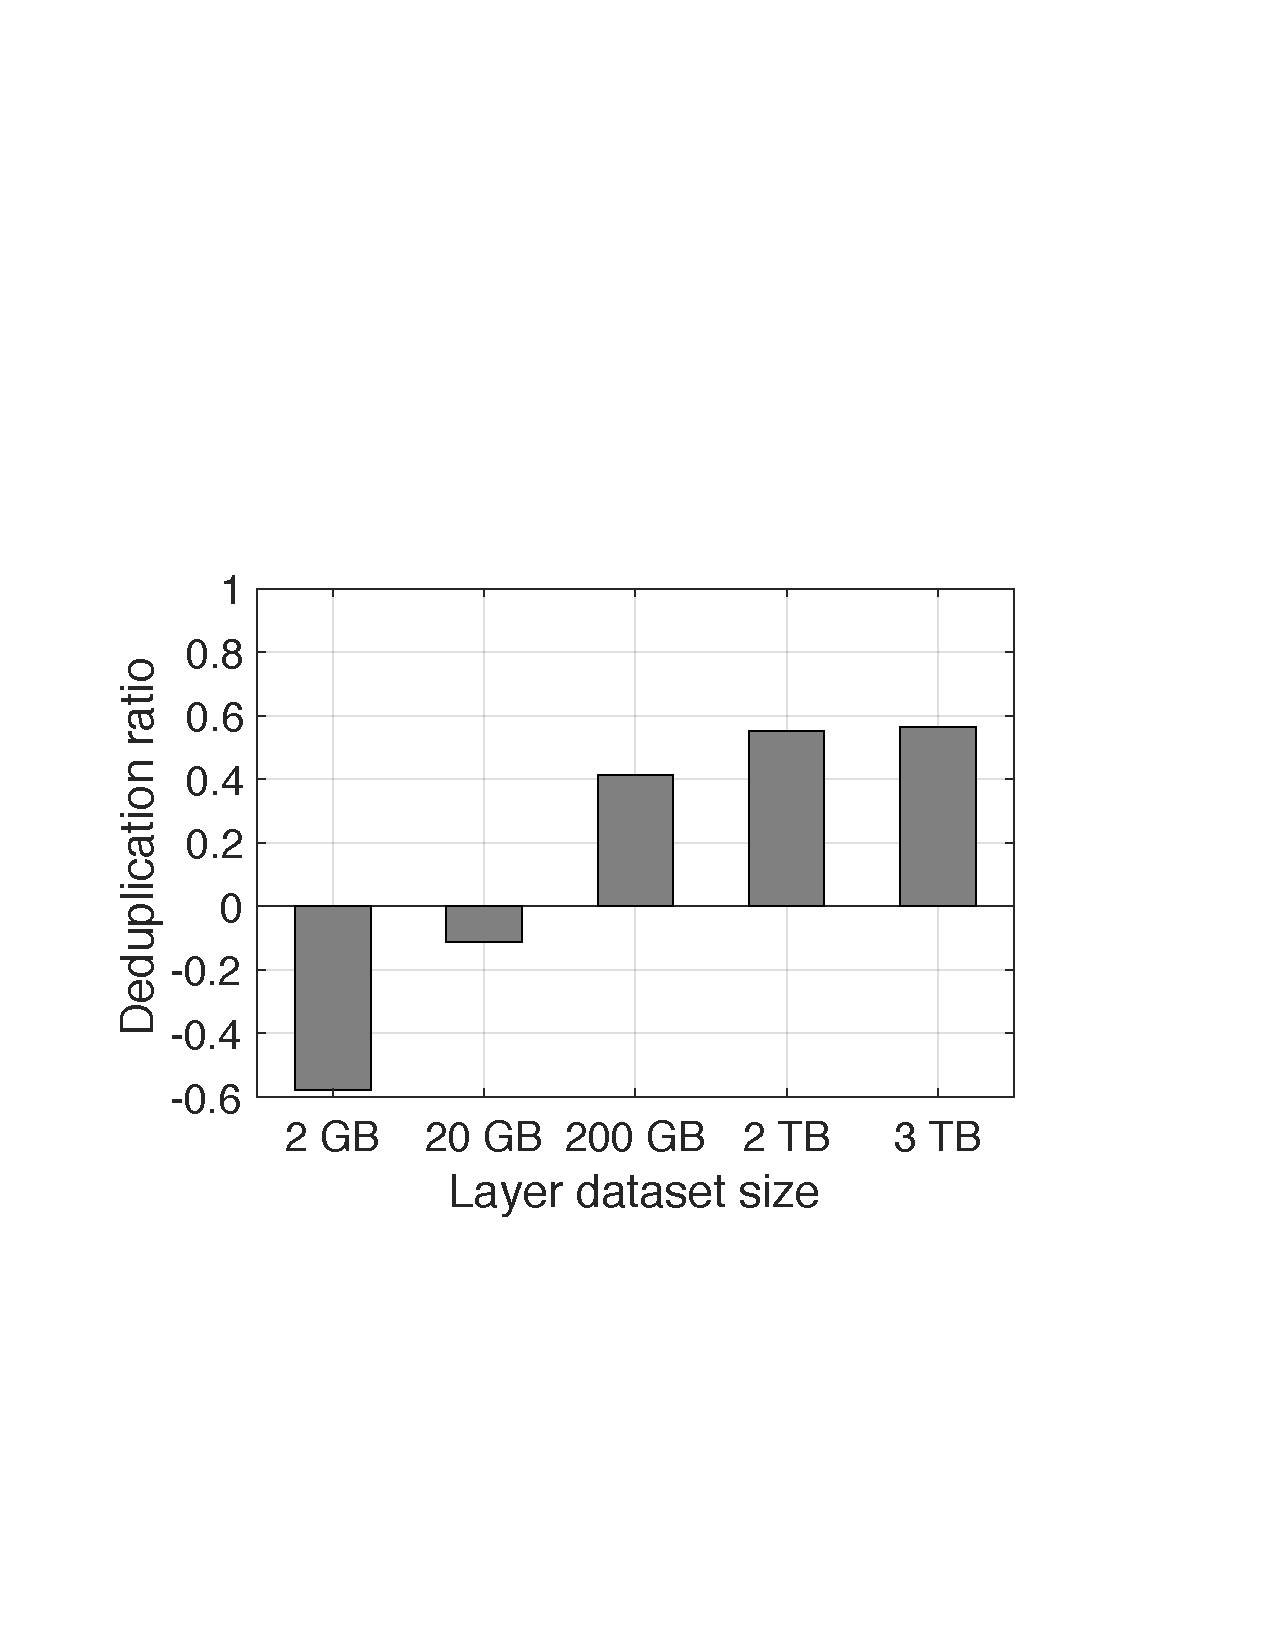
\includegraphics[width=1\textwidth]{graphs/dedup_vs_compression.pdf}
			\caption{File-level deduplication vs. compression efficiency.}
		%	\vspace{-3pt}
			\label{fig:cacheefficiency}
		\end{minipage}
			\begin{minipage}{0.38\linewidth}
				\centering
				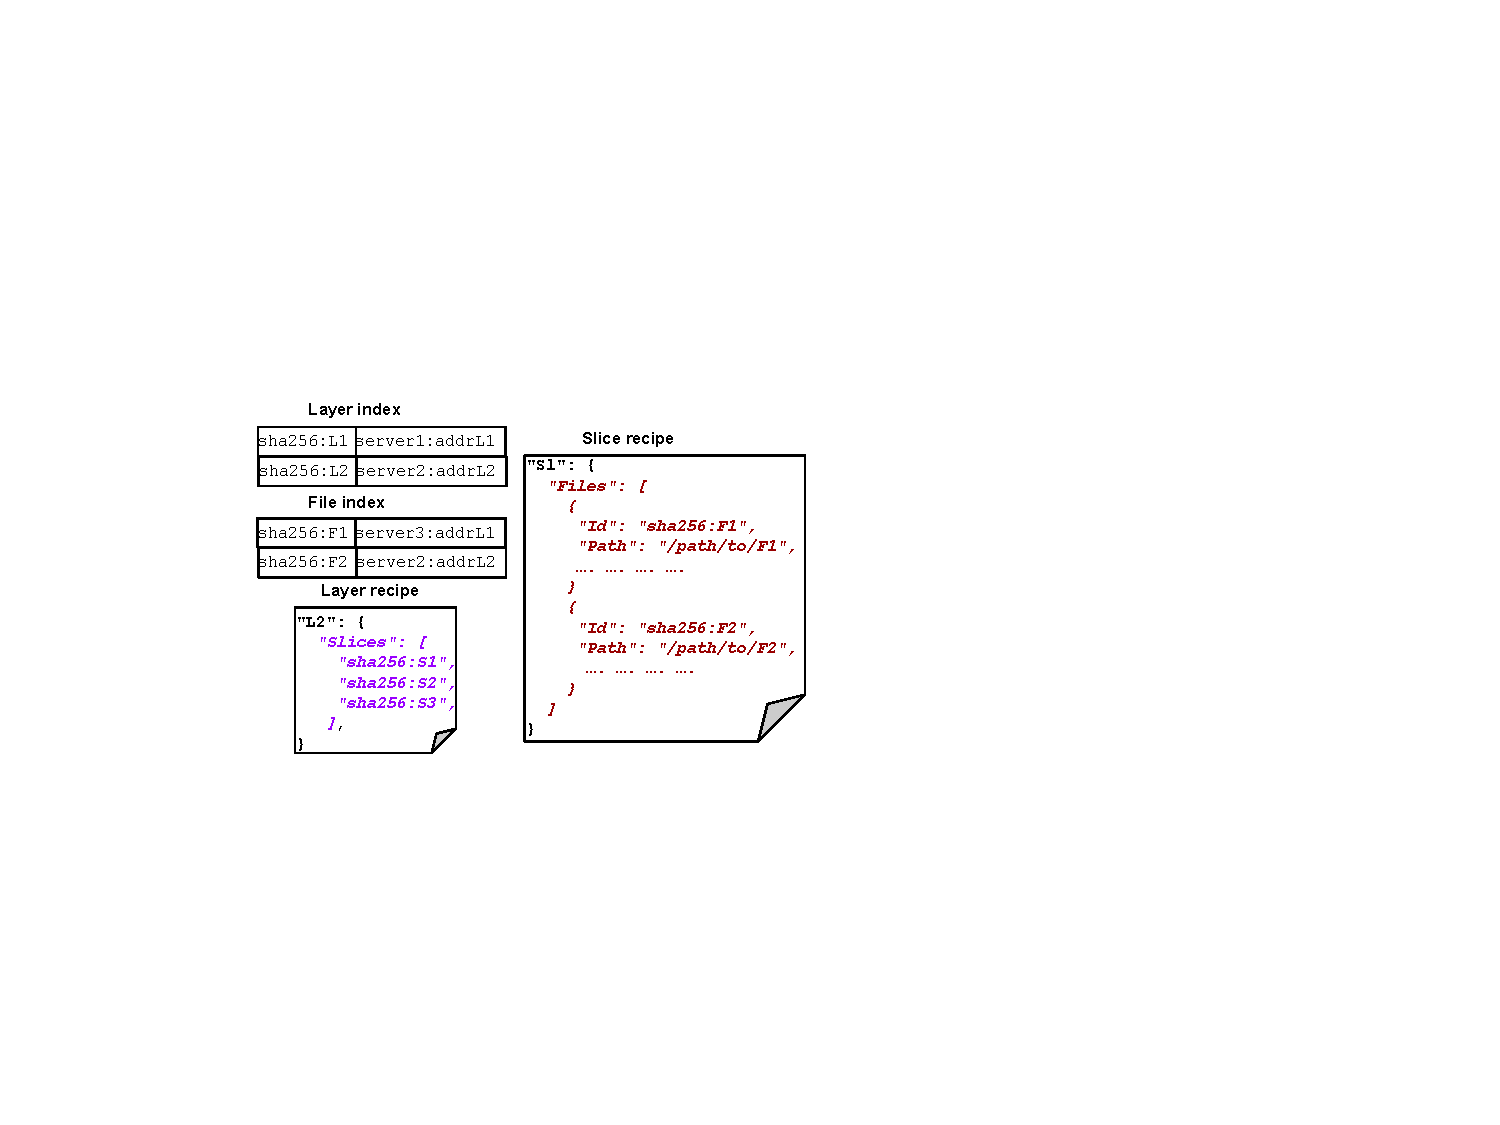
\includegraphics[width=1\textwidth]{graphs/sift-metadata.pdf}
				\caption{Metadata for deduplication.}
				%	\vspace{-3pt}
				\label{fig:sift-metadata}
			\end{minipage}
		\begin{minipage}{0.38\linewidth}
			\centering
			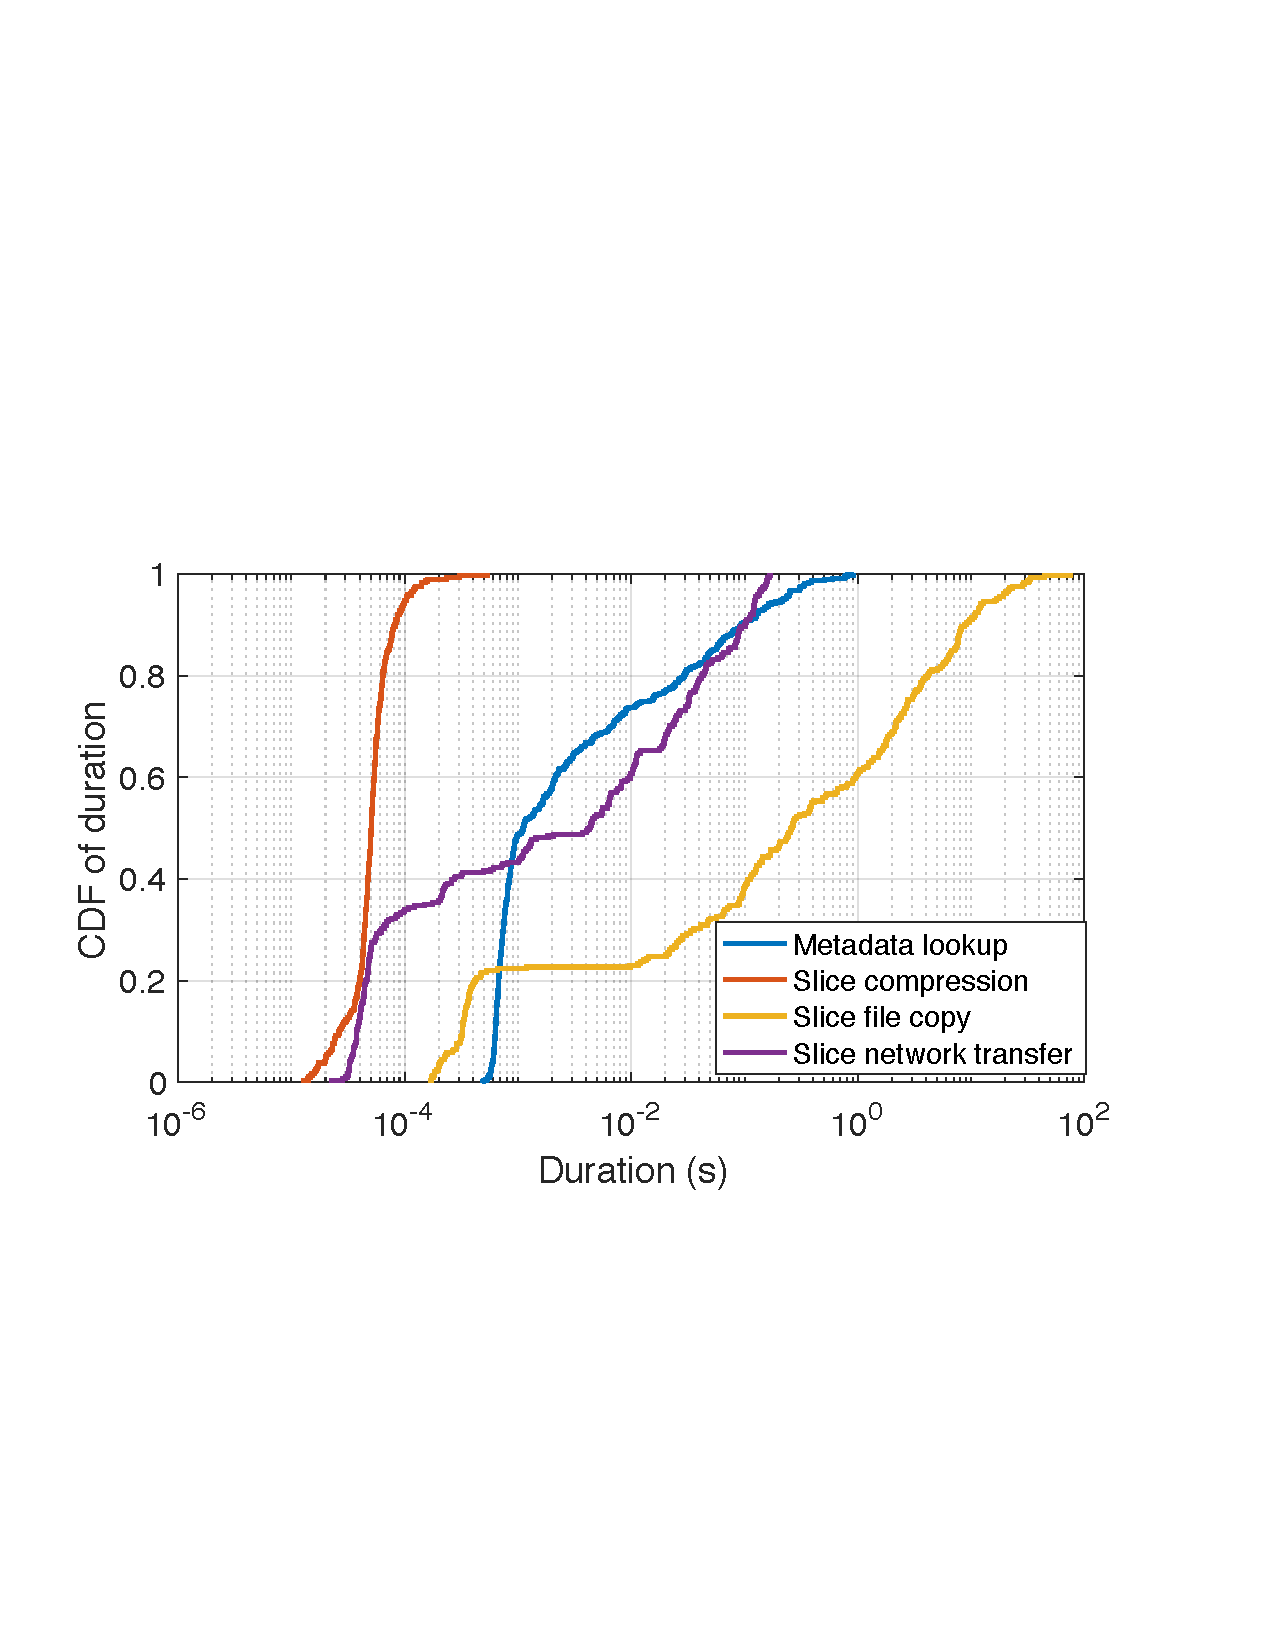
\includegraphics[width=1\textwidth]{graphs/restoring-breakdowns.pdf}
			\caption{Breakdown of slice restoring time.}
			%	\vspace{-3pt}
			\label{fig:slice-restoring-breakdown}
		\end{minipage}
\end{figure*}

%\begin{figure}[t]
%	\centering
%	\begin{minipage}{0.26\textwidth}
%		\centering
%		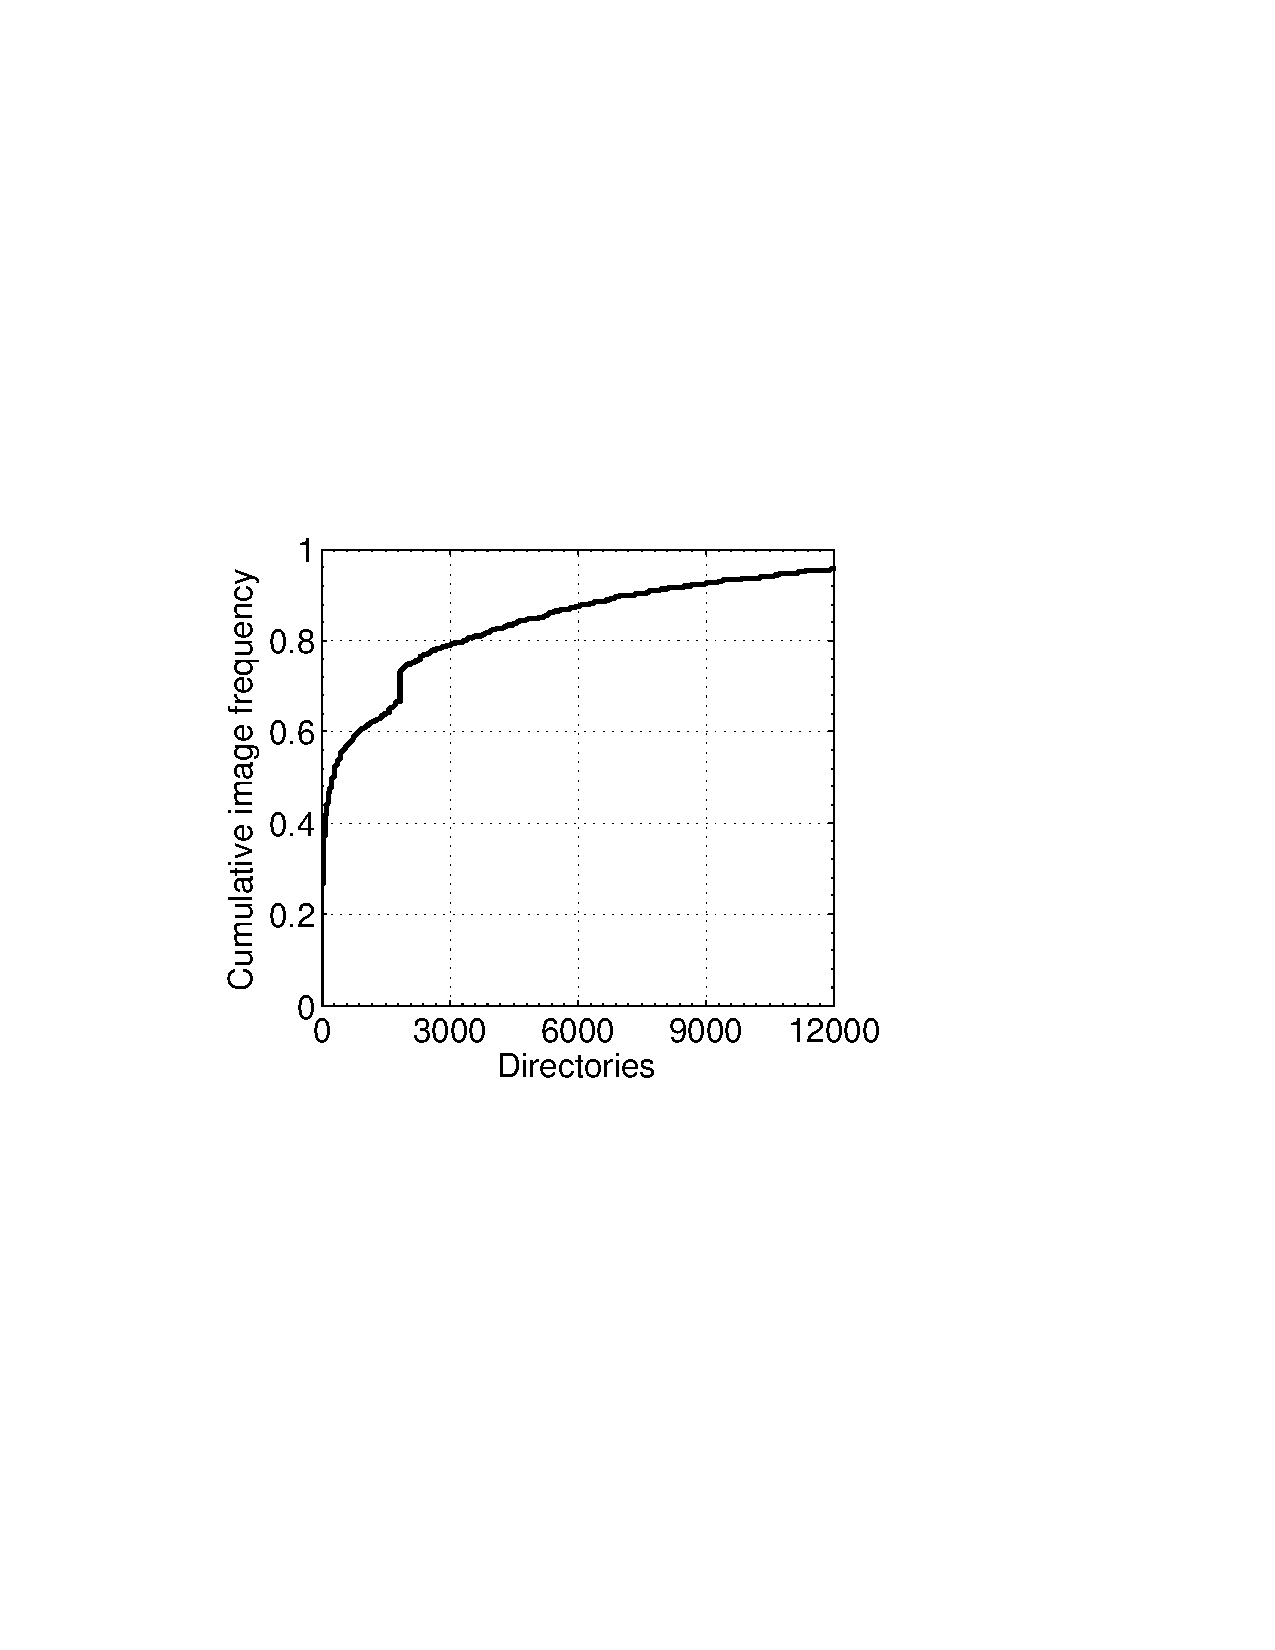
\includegraphics[width=1\textwidth]{graphs/dir.pdf}
%		\caption{CDF of images by\newline directories}
%		\label{fig-dir}
%	\end{minipage}%
%	\begin{minipage}{0.24\textwidth}
%		\centering
%		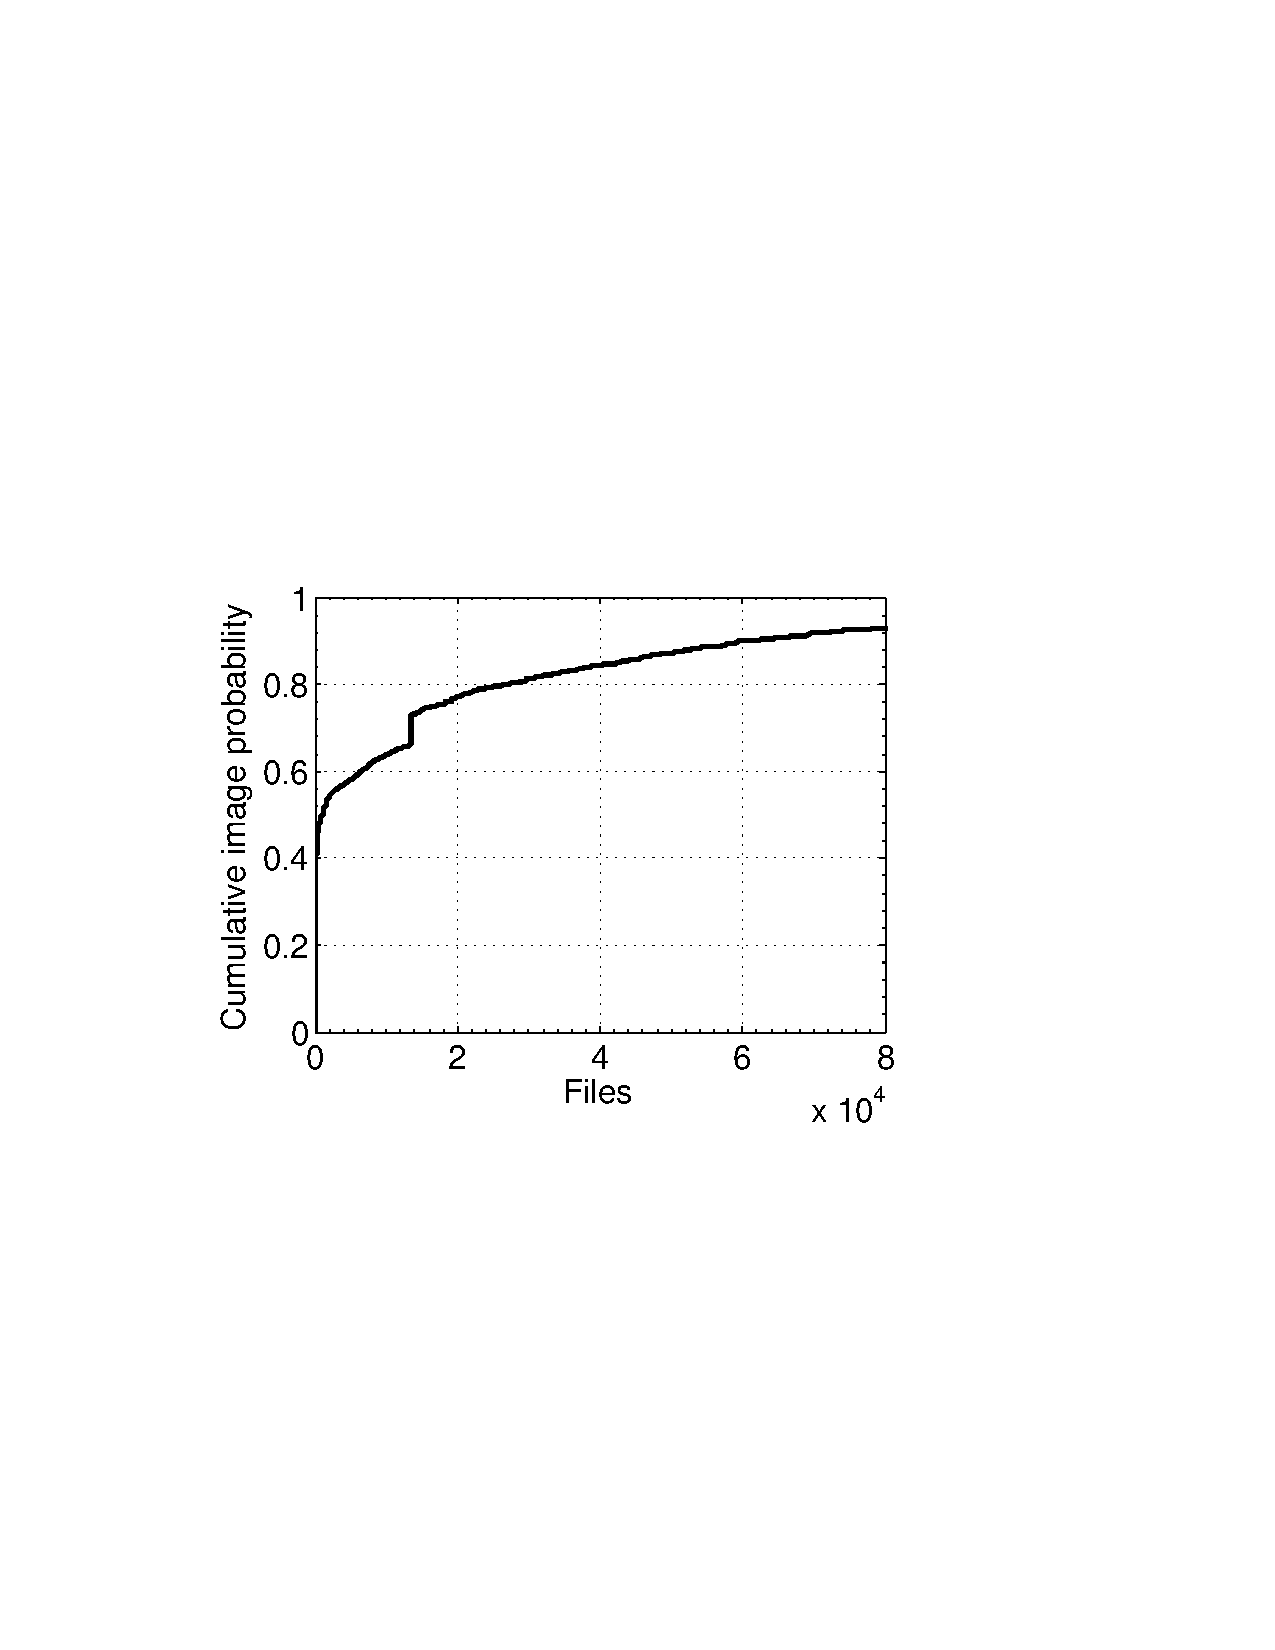
\includegraphics[width=1\textwidth]{graphs/file.pdf}
%		\caption{CDF of images by files}
%		\label{fig-file}
%	\end{minipage}
%\end{figure}

%\begin{figure}[htbp] 
%	\begin{minipage}{0.5\linewidth} 
%		\centering 
%		\includegraphics{circle} 
%		\caption{A Circle} 
%		\label{fig:circle} 
%	\end{minipage}% 
%	\begin{minipage}{0.5\linewidth} 
%		\centering 
%		\includegraphics{rectangle} 
%		\caption{A Rectangle} 
%		\label{fig:rectangle} 
%	\end{minipage} 
%\end{figure}

Consider that deduplication incurs a performance overhead 
and the current Docker registry already stores layers in compressed format to 
save space and network transfer overhead. 
We first analyze the space efficiency of a registry 
 that performs decompression and file-level deduplication and compare it to 
 a registry that naively stores compressed layers.

In Figure~\ref{fig:cacheefficiency}, the x-axis values correspond to the sizes of $5$ random samples 
drawn from the whole dataset (detailed in~\cref{sec:dataset-analysis}). %and the size of the dataset in terms of capacity and layer count.
For a traditional registry, the compressed layer tarballs will be kept as is.
While a registry with file-level deduplication will store \emph{deduplicated} layers (i.e., unique files). 
The y-axis shows how much space a registry with file-level deduplication can save compared to naively storing compressed layer tarballs.
For the first two samples of the dataset, with size less than $20$~GB, 
there is no benefit to \emph{deduplicate} layers 
because the deduplication ratio is very low.
However, when the dataset size is $3$~TB, we can save $56\%$ more space.
The space saved by applying decompression and file-level deduplication increases almost linearly with the size of the layer dataset.
This verifies the benefit of deduplicate layers when the dataset is large, 
which should be carefully selected to realize significant space savings.

\subsubsection{Layer deduplication}

After receiving a \texttt{push} layer request, \sysname~will store the layer as it is and return a response back to client. 
\dedupname system~initiates layer deduplication process only if 
layer deduplication will achieve significant space savings and 
the process won't impact foreground requests. 
Sepcially, layer deduplication process is triggered when
the layer dataset $S$ is greater than a predefined threshold $\theta_{s}$ and 
the registry traffic $RPS$ ( i.e., requests per second) is lower than $\theta_{RPS}$. Thus, layer deduplication process runs periodically.
The process always stars with the cold layers that haven't been
access for a long time.
  
The deduplication process has tree major steps: layer decompression, file-level deduplication,
and unique file distribution. 
The first two steps are necessary for removing file duplicates from compressed layer tarballs.
The last step -- unique file distribution is to balance the layer restoring load among registries so that 
layer restoring process will achieve an optimal parallelism for each layer (detailed in~\cref{subsubsec:slice-restoring}) 
and 
accelerate layer restoring process. 
%After layer deduplication, unique files are evenly distributed across multiple registry servers. 
%We define all the per-server files belonging to a layer as a {\em slice}. 
%A server stores slices for many layers, and a layer is composed of slices stored on multiple servers, which allows restoring a layer in parallel. 

%\begin{figure}[t]
	\centering
%		\begin{minipage}{0.23\textwidth}
%			\centering
%			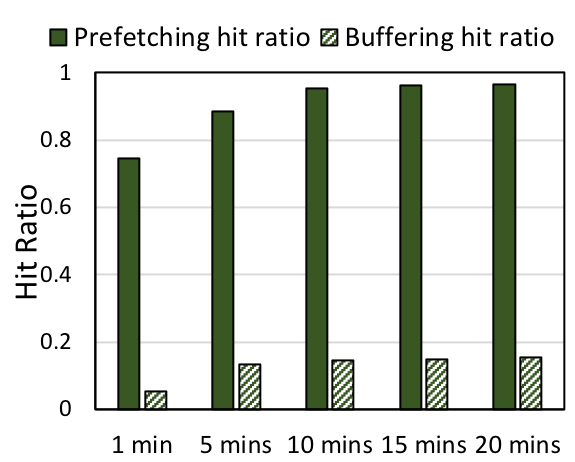
\includegraphics[width=1\textwidth]{graphs/evaluation_hitratios.png}
%			\caption{Hit ratio.}
%			\label{fig:hitratio}
%		\end{minipage}
	%	\begin{minipage}{0.25\textwidth}
			\centering
			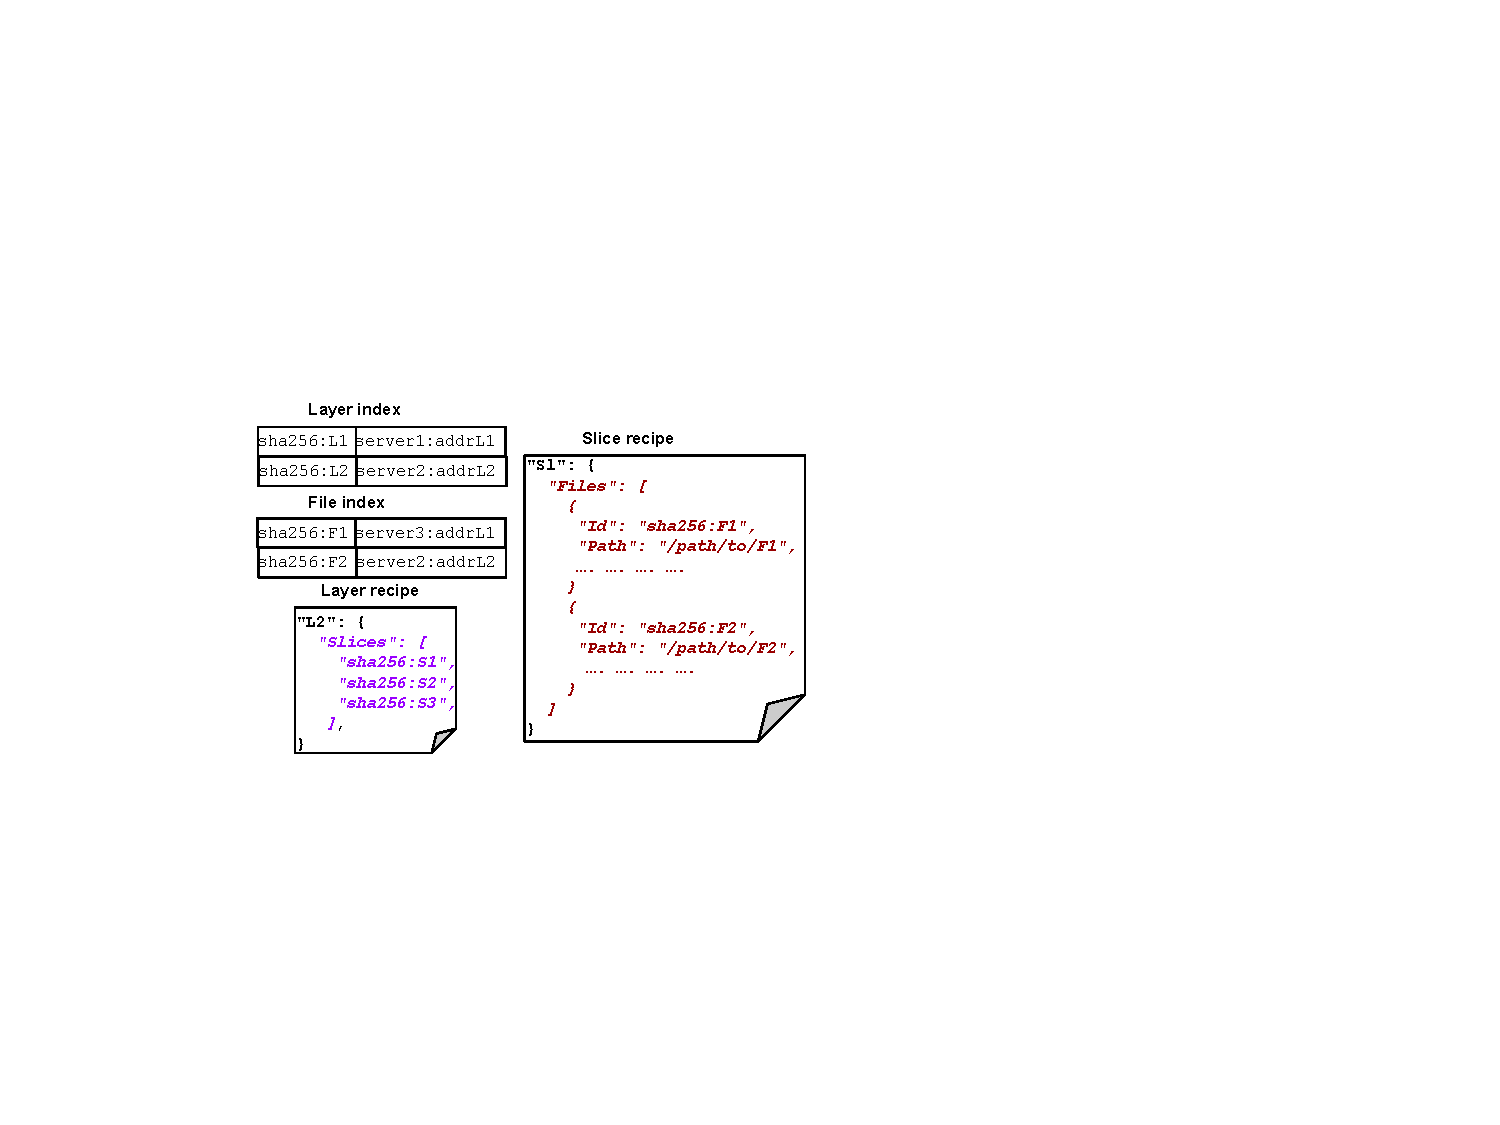
\includegraphics[width=0.4\textwidth]{graphs/sift-metadata.pdf}
			\caption{Metadata for deduplication.}
			%\vspace{-3pt}
			\label{fig:sift-metadata}
	%	\end{minipage}
\end{figure}
Similar with traditional registry, 
\dedupname~system maintains layer index to address the corresponding layers stored in the system
as shown in Figure~\ref{fig:sift-metadata}.
The deduplication process first checks the layer fingerprint in the \emph{layer index} to ensure 
an identical layer is not already stored. Then,
\dedupname~system decompresses and unpacks the unique layer into files.
Next, 
it computes a \emph{fingerprint} for every file in the slices
and checks every file's fingerprint in the \emph{file index} to get identical files' server addresses.
After that, it uses a weighted round robin algorithm to distribute newly added 
unique files to the registry cluster. These servers that already contains this layer's identical files
are assigned a lower weight. 
This is to ensue that different servers maintain same amount of files that are needed to restoring equal sized 
slices for this layer.
Deduplication process also 
updates the \emph{file index} with the newly added unique files' fingerprints and host addresses.   
Then, it calculates the slice fingerprints and creates a slice recipe for each slice.
Slice recipe contains partial of the layer tarball's directory tree structure, file fingerprints, file name along with file path in the tarball, and file metadata information 
(such as permissions and creation date), which are needed for restoring a slice for the layer. 
Note that, layer deduplication process only deduplicates regular files.
%After that
%After removing the duplicate files,
%Then, it
%distributes the \emph{deduplicated slices} evenly to the registry cluster by using round-robin, and,
In the end, deduplication process creates a layer recipe which contains its slices' fingerprints and 
based on layer recipe, it updates image manifests.
The layer's tarball and file duplicates are removed after deduplication.

\paragraph{Parallel slice restoring}
\label{subsubsec:slice-restoring}

When a~\texttt{pull slice}~request is received, the \dedupname~system 
first prepares a directory structure for the slice, based on the slice recipe.
Then, it copies the files into the directory tree.
Next, it compresses the slice's directory tree into a slice tarball,
and directly sends it back to the client.

\subsubsection{Layer restoring assisted file cache (LRA file cache)}

Slice restoring process has four suboperations: 
slice recipe lookup,
slice file copying,
slice compression, and
slice network transfer. 
To measure the overhead for each suboperation, 
we implemented layer deduplication and parallel slice
restoring on a 4-node registry cluster. 
We first warmup the cluster by pushing 200 layers to the cluster
and initiating layer deduplication process.
The layers were randomly selected from our layer dataset detailed in xxx limited to 50MB.
After finishing layer deduplication,
we sent 400 \texttt{pull slice} requests to the cluster with 10 \texttt{pull slice} requests issued at a time.
Figure~\ref{fig:slice-restoring-breakdown} shows the CDFs of the latencies for each suboperation.
We see that across the four suboperations,
the duration for slice compress is the shortest.
Slice compression only took less than 0.001 s because a slice is a smaller unit. 
The next shortest suboperation is network transfer since we pulled layer slice through Ethernet.
90\% of slice recipe lookups took less than 0.1 s while 
the highest slice recipe lookup duration almost reaches 0.8 s,
which is caused by high concurrent lookup requests 
%(note that we use redis to store metadata \NZ{use mongodb instead}).
The most time consuming suboperation is slice file copying, which involves 
copying all 
the files that belong to the slice to their destination directory based on the slice recipe.
Note that we implemented a thread pool on each registry server to read files in parallel
and write data in RAMdisk to reduce disk IOs.
40\%of slice file copying duration is greater than 1 s and 
10\% of slice file copying duration is higher than 10 s.
This is because bigger slices contains more files and requires more disk IOs.
The overhead of slice copying can be largely mitigated for a large-scale registry cluster
since the size of slice roughly equals to $S_{l}/N$, where $S_{l}$ denotes the layer size and $N$ is size of registry cluster.
However, it could be a bottleneck for slice restoring on a small-scale registry cluster.
%and slice file copying duration depends on slice size.

\begin{algorithm}
\scriptsize 
	\caption{File cache assisted slice restoring}
	\label{alg:file-cache}
	\KwIn{\\
		$\theta_{rsfc}$: Slice restoring latency threshold. \\
		$s$: Slice to be restored. \\
	}

	\SetKwFunction{Fsub}{Restore}
	\SetKwProg{Fn}{Function}{:}{}

	\Fn{\Fsub{s}}{
		%{\tiny\texttt{/* Otherwise, it's a repull layer miss   /}}\\
		\eIf{files in s are cached in file cache}
		{
			slice $\gets$ \texttt{RestoreSlice} \emph{s} \texttt{From} \emph{file cache + disk} 
		}
		{
			slice, $D_{rs}$ $\gets$ \texttt{RestoreSlice} \emph{s} \texttt{From} \emph{disk} \\
			\If{ $D_{rs} > \theta_{rsfc}$} 
			{ 
				\emph{file cache} $\gets$ \texttt{Cache} \texttt{Subsetof} \emph{s.files}
			}		
		}
	}

\end{algorithm}




To reduce slice file copying overhead,
\sysname~\filecachename~temporally cache a subset of unique files for bigger and popular slices that have a high slice restoring latency, ie., $D_{rs} > \theta_{rsfc}$, 
where $D_{rs}$ is the slice restoring latency and $\theta_{rsfc}$ is the restoring latency threshold for 
caching
a subset of files from the slice to help improve its restoring performance as shown in Algorithm~\ref{alg:file-cache}.
Upon a \texttt{pull slice} request for those slices, 
\dedupname~ system fetches a subset of its containing files from \filecachename~and
the remaining files from disk for slice restoring.

To identify which slices have a high slice restoring latency,
\dedupname~system monitors slice restoring performance and 
maintains a restoring performance  profile for each slice that has been restored,
% as shown in Figure~\ref{fig:xxx},
which contains the latency breakdown of slice restoring
% (,and a decompression latency updated by layer decompression process) 
and its containing files' sizes.
All the slice restoring performance profiles are also stored in distributed  databases,
 and addressed by slice digests. 
To estimate the restoring latency for a slice $i$ that hasn't been restored, 
\dedupname system~first lookups the slice restoring performance profiles by slice size,
 then selects a slice $x$ that is most similar in size to $i$,
 and estimates $i$'s restoring latency as: 
 $D_{rs}(i) \approx D_{rs}(x) + \Phi_{rs}(\Delta_{S})$,
 where $\Delta_{S}$ is the size different between two slices.
 $\Phi_{rs}(\Delta_{S})$ denotes a slice restoring latency function of slice size variation.
  $\Phi_{rs}(\Delta_{S})$ is generated by using linear regression~\cite{xxx}.
 %$\varepsilon_{rs}$ is the standard error of restoring latency estimation for the layers similar in size.
If the estimated slice restoring $D_{rs}(i) > \theta_{rs}$,
then, \dedupname~lookups the slice restoring performance profiles by slice size,
selects a slice $y$ that has a acceptable restoring latency and
most similar in size to $i$.
Next, \dedupname system~caches a subset of files $F$ for slice $i$, so that
$D_{rs}(i) - \Phi_{rs}(\Sigma_{S}(F)) \approx D_{rs}(y)$,
where $\Sigma_{S}(F)$ is the sum size of files in $F$.

Note that \filecachename~size is limited so that \filecachename~only caches 
subsets of files for big slices that belongs to popular layers.
%that will be accessed later. 
\cref{sec:cache-design} will describe how to determine popular layers based on user access patterns.
Note that the slices for the same layer have similar sizes, restoring latencies, and popularity 
because of unique file
distribution. 
Thus, once a layer is determined as popular layer, 
\dedupname~will cache similar amount of files for its slices.
Note that all the files in file cache are unique and can be shared for restoring different slices.

For on-premise or private registry cluster, the network transfer speed is usually faster than remote cloud.
Thus, slice compression is less important for medium to small size slices, 
especially for the slices that have a high decompression latency, 
i.e., $D_{stt} < \theta_{stt}$ and $D_{dc} > \theta_{dc}$, where $D_{stt}$ and $D_{dc}$ denote slice transfer duration
and decompression duration respectively; 
$\theta_{stt}$ and $\theta_{dc}$ denote thresholds for them respectively.
Consequently, \dedupname system~only archives these slices without compressing them and directly sends
these archival files back to the clients to eliminate clients' decompression latency.



